\documentclass{article}

\usepackage{fancyhdr}
\setlength{\headheight}{12pt}
\setlength{\textwidth}{17.2cm} \setlength{\textheight}{23cm}
\setlength{\topmargin}{-2.5cm} \setlength{\headsep}{1.6cm}
\setlength{\evensidemargin}{-.8cm}
\setlength{\oddsidemargin}{-.8cm}
%\pagestyle{fancy}

%set-up page dimentions
\usepackage[top=1 in, bottom = 1 in ,left = 1.5 in, right = 1.5in]{geometry}

\setlength{\parskip}{12pt}  % 12 pt = space between paragraphs
\setlength{\parindent}{12pt} % 0 pt  = indentation
\usepackage{amsmath}
\usepackage{amssymb}
\usepackage{amsthm}
\usepackage{ifthen}
\usepackage{latexsym}
\usepackage{graphicx}
\usepackage{graphics}
\usepackage{psfrag}
\usepackage{graphpap}

\newcommand{\conman}{\texttt{ConMan }}


% Allows hyperlinks if compiled with pdflatex
\usepackage{hyperref}
\hypersetup{colorlinks}
\usepackage{color}
\definecolor{darkred}{rgb}{0.5,0,0}
\definecolor{darkgreen}{rgb}{0,0.5,0}
\definecolor{darkblue}{rgb}{0,0,0.5}
\hypersetup{ colorlinks,
                linkcolor=darkblue,
                filecolor=darkgreen,
                urlcolor=darkblue,
                citecolor=darkblue }
%hyperlink example is: \href{http://www.google.com}{google}

%add code!
\usepackage{listings}
\definecolor{mygreen}{rgb}{0,0.6,0}
\definecolor{mygray}{rgb}{0.5,0.5,0.5}
\definecolor{mymauve}{rgb}{0.58,0,0.82}
\lstset{ %
backgroundcolor=\color{white},   % choose the background color; you must add \usepackage{color} or \usepackage{xcolor}
basicstyle=\footnotesize,        % the size of the fonts that are used for the code
breakatwhitespace=false,         % sets if automatic breaks should only happen at whitespace
breaklines=true,                 % sets automatic line breaking
captionpos=b,                    % sets the caption-position to bottom
commentstyle=\color{mygreen},    % comment style
deletekeywords={...},            % if you want to delete keywords from the given language
escapeinside={\%*}{*)},          % if you want to add LaTeX within your code
extendedchars=true,              % lets you use non-ASCII characters; for 8-bits encodings only, does not work with UTF-8
frame=single,                    % adds a frame around the code
keepspaces=true,                 % keeps spaces in text, useful for keeping indentation of code (possibly needs columns=flexible)
keywordstyle=\color{blue},       % keyword style
language=Octave,                 % the language of the code
morekeywords={*,...},            % if you want to add more keywords to the set
numbers=none,                    % where to put the line-numbers; possible values are (none, left, right)
numbersep=5pt,                   % how far the line-numbers are from the code
numberstyle=\tiny\color{mygray}, % the style that is used for the line-numbers
rulecolor=\color{black},         % if not set, the frame-color may be changed on line-breaks within not-black text (e.g. comments (green here))
showspaces=false,                % show spaces everywhere adding particular underscores; it overrides 'showstringspaces'
showstringspaces=false,          % underline spaces within strings only
showtabs=false,                  % show tabs within strings adding particular underscores
stepnumber=2,                    % the step between two line-numbers. If it's 1, each line will be numbered
stringstyle=\color{mymauve},     % string literal style
tabsize=2,                       % sets default tabsize to 2 spaces
title=\lstname                   % show the filename of files included with \lstinputlisting; also try caption instead of title
}


\begin{document}
\begin{titlepage}
\Huge
\vspace{2cm}
\begin{center}
Software Design Document for the \texttt{ConMan}\\
\vspace{3cm}
\Large
Authors:\\ 

\begin{tabular}{l l}\hline
 & \\
 & 
\end{tabular}
\vspace{1cm}

Version 0.1\\
10/28/2013
\end{center}


\end{titlepage}

\normalsize

\newpage
\tableofcontents

\newpage
\section{Introduction}
This software design document provides a description of the \texttt{ConMan} application.  In addition to describing the basic user interface design, the client-server interface and database description are also provided here.

\subsection{Goal and Purpose}
The purpose of \texttt{ConMan} is to provide a simple, web-based task-management application that can be used by both individuals and teams. The user interface should be easy to learn without hiding any of the core features of \texttt{ConMan}. The applications and its data should be protected with controls such as permission checking to ensure that data is not leaked and/or corrupted. 

\subsection{Core Features}
The core features of \texttt{ConMan} include:
\begin{itemize}
\item Ability to register as a user
\item Ability to define teams of users
\item Ability to create, view, update, and delete project tasks
\item Ability to create, view, update, and delete checklists associated with tasks
\item Ability to register for notifications (via the application and via email) of upcoming deadlines
\item Ability to view deadlines through a calendar interface
\end{itemize}

\subsection{Major Constraints}
The most limiting constraint is time. Due to time constraints, all development and testing must be completed within a 2 month period. Another constraint relates to the team's web development experience. Some on the team has little web development experience and even lower experience with the technologies that will be used (ASP.NET, jQuery, etc.).

\subsection{Intended Audience and Reading Overview}
This document is intended for individuals involved in the design and implementation of the \texttt{ConMan} web application. Stakeholders and customers may also want to read this document with the goal of ensuring that the product is being developed to their requirements. This document can be read in a sequential manner or by individual sections in any order. Below is a list of sections along with a short description:
\begin{itemize}
\item Architectural Design (Section 2)
\begin{itemize}
\item The two major components of \texttt{ConMan}`s Client-Server architecture are discussed.
\end{itemize}
\item Data Design (Section 3)
\begin{itemize}
\item The database tables are defined and the data transactions are described.
\end{itemize}
\item User Interface Design (Section 4)
\begin{itemize}
\item The general layout for the main page of the web application is depicted through the use of multiple wireframes.
\end{itemize}
\item Restrictions, Limitations, and Constraints (Section 5)
\begin{itemize}
\item This section specifies the browsers to be supported by the initial release of ConMan and the application's reliance on internet connections.
\end{itemize}
\item Testing Guidelines (Section 6)
\begin{itemize}
\item A variety of test cases are presented along with their expected results. 
\end{itemize}
\item Appendices (Section 7)
\begin{itemize}
\item This section contains a list of definitions of terms used throughout the document.
\end{itemize}
\end{itemize}
\newpage
\section{Architectural Design}
\subsection{Overview}
\texttt{ConMan} is divided into two major components: the client-side user interface, and a server-side application and database.
The client-side communicates with the server using HTTP requests sent through an internet browser.  
\texttt{ConMan} utilizes the Client-Server architecture and allows multiple clients to concurrently access the server.  

\subsection{Client-Server Interaction}
Data and user interactions are passed between the database, server, and clients through a MVC architecture.

The \texttt{ConMan} database will maintain the data for the \texttt{ConMan} application.  
The database will have no direct interaction with the clients and is only accessible through an interface with the server.
Requests made to the database will occur in a First-Come, First-Served manner in order to preserve data consistency.

The \texttt{ConMan} server parses HTTP requests made by the clients and will interface with the database as needed.  
The server itself will be stateless and will not maintain user or application data after a request is handled.
Data passed between the client and server will be in the JSON format.

\subsection{Basic Context}
The "basic context" of \texttt{ConMan} is where a user can only take actions that affect their personal account.
Every \texttt{ConMan} user has a basic account, and consists of the tasks and checklists that are not a part of external teams or groups.
When a user opens the \texttt{ConMan} application by pointing their browser to the \texttt{ConMan} URL, the initial user context is the basic context.
The basic context is also the starting context when an account is created.


\subsubsection{Interface Description}
Fields entirely enclosed in [] brackets are to be considered optional.
\begin{lstlisting}
CreateAccount(  LastName:String,
                FirstName:String,
                E-mail:String,
                Password:String);
\end{lstlisting}

\begin{lstlisting}
ModifyAccount(  UserId:Int,
                [LastName:String],
                [FirstName:String],
                [E-mail:String],
                [NewPassword:String],
                OldPassword:String);
\end{lstlisting}

\begin{lstlisting}
CreateTask( UserId:Int,
            TeamId:Int,
            DueDate:date,
            Description:String);
\end{lstlisting}

\begin{lstlisting}
ModifyTask( UserId:Int,
            TaskId:Int,
            TeamId:Int,
            [DueDate:date],
            [Description:String],
            [Completed:Boolean],
            [Note:String]);
\end{lstlisting}

\begin{lstlisting}
CreateChecklist(    UserId:Int,
                    TeamId:Int,
                    TaskId:Int,
                    DueDate:date,
                    Fields:[{CheckListId:Int, FieldId:Int DueDate:date, Description:String}],
                    Description:String);
\end{lstlisting}

\begin{lstlisting}
ModifyChecklist( UserId:Int,
                 CheckListId:Int,
                 TaskId:Int,
                 [DueDate:date],
                 [Description:String],
                 [Fields:[{CheckListId:Int, FieldId:Int DueDate:date, Description:String}]],
                 [CompletedField:Boolean[]],
                 [Completed:Boolean],
                 [Note:String]);
\end{lstlisting}

\subsubsection{Processing Details}
The \texttt{CreateAccount} interface is used when the user first creates an account with the \texttt{ConMan} system.
The server will validate the input fields given by the user.
If all fields are valid, the server will update the database records and add a new user.
A team is automatically generated with a team-Id equivalent to the user-Id.
If the server successfully validates the user fields and successfully updates the database, the user-Id generated by the database will be returned.
Otherwise, an error code will be returned.

\texttt{ModifyAccount} functions similarly to \texttt{CreateAccount}, except fields that \texttt{NULL} can be given for fields that are not being updated and are not required to identify the action.

\texttt{CreateTask} adds a new task for the user. 
In the basic context, the \texttt{TeamId} will be the \texttt{UserId}. 
After verification by the server and a successful database update, the task-Id will be returned.
Otherwise, an error code will be returned.

\texttt{ModifyTask}, like \texttt{ModifyAccount} allows texttt{NULL} values to be given for fields that are not being updated.
A success or error code will be returned.

\texttt{CreateChecklist} will add a checklist to a task owned by a user.
In the basic context, the \texttt{TeamId} will be the \texttt{UserId}.

\texttt{ModifyChecklist} This interface function is invoked to modify an existing checklist.
 
\subsubsection{Restrictions/Limitations}
For every interface action, the server must validate the given fields against the database to ensure the user making the request has the appropriate permissions.
\subsubsection{Performance Issues}
Requests made by the clients to the server are subject to time-out restrictions.  
If the server takes too long to process an interface request and the client-server connection is ended, the client will assume the transaction failed.
Under such a failure condition, the client will send a "revoke" notice to the server indicating that any database changes made on behalf of the timed-out request must be rolled-back.
\subsubsection{Design Constraints}
In order to maintain data consistency, either only one database should be used, or a very robust data-duplicating effort must be made to ensure consistency across multiple databases.  
Version one of \texttt{ConMan} will only support a single database back-end.

\subsection{Team Context}
The team context is conceptually very similar to the basic context, except administrator privileges are required to modify the team account.
Administrator privileges are automatically given to the creator of a team.
Tasks associated with the team can be modified by all team administrators and all users belonging to the team who have been assigned to the task.

\subsubsection{Interface Description}
Fields entirely enclosed in [] brackets are to be considered optional.
\begin{lstlisting}
CreateTeam(     TeamName:String,
                E-mail:String,
                Password:String);
\end{lstlisting}

\begin{lstlisting}
ModifyTeam(     TeamId:Int,
                [TeamName:String],
                [E-mail:String],
                [NewPassword:String],
                OldPassword:String);
\end{lstlisting}

\begin{lstlisting}
CreateTeamTask( UserId:Int,
                TeamId:Int,
                AssignedUsers:Int[],
                DueDate:date,
                Description:String);
\end{lstlisting}

\begin{lstlisting}
ModifyTeamTask( UserId:Int,
            TaskId:Int,
            TeamId:Int,
            [AssignedUsers:Int[]],
            [DueDate:date],
            [Description:String],
            [Completed:Boolean],
            [Note:String]);
\end{lstlisting}

\begin{lstlisting}
CreateTeamChecklist(    UserId:Int,
                        TeamId:Int,
                        TaskId:Int,
                        AssignedUsers:Int[],
                        DueDate:date,
                        Fields:[{CheckListId:Int, FieldId:Int DueDate:date, Description:String}],
                        Description:String);
\end{lstlisting}

\begin{lstlisting}
ModifyTeamChecklist( UserId:Int,
                 CheckListId:Int,
                 TeamId:Int,
                 TaskId:Int,
                 [AssignedUsers:Int[]],
                 [DueDate:date],
                 [Description:String],
                 [Fields:[{CheckListId:Int, FieldId:Int DueDate:date, Description:String}]],
                 [CompletedField:Boolean[]],
                 [Completed:Boolean],
                 [Note:String]);
\end{lstlisting}

\subsubsection{Processing Details}
The processing details for the team context differ from the basic context only in the fact that an additional check must be performed to ensure the user making the request has the correct team permissions to do so.
\subsubsection{Restrictions/Limitations}
There are no additional restrictions or limitations.
\subsubsection{Performance Issues}
There are no additional performance constraints.
\subsubsection{Design Constraints}
There are no additional design constraints.

%
%\subsection{Group Administrator}
%
%\subsubsection{Interface Description}
%\subsubsection{Processing Details}
%\subsubsection{Restrictions/Limitations}
%\subsubsection{Performance Issues}
%\subsubsection{Design Constraints}
%
%


\newpage
\section{Data Design}
The server-side database provides persistent data storage for the \texttt{ConMan} application.
When a user connects to the \texttt{ConMan} application through a web-browser, the data associated with that user is retrieved by the server from the database and sent as a JSON encoded string back to the user for client side processing.
To preserve consistency, client-side processing will only handle representation of the data (i.e. the "view").
Any create, update, or destroy operations on the data must be validated by a server request (interfaces defined below).

All data held outside of the database - client and server-side -  will not be preserved by the \texttt{ConMan} application when the user navigates away from the \texttt{ConMan} page.

\subsection{Database Design}
The following database table descriptions describe the data interactions and dependencies.

\begin{tabular}{|l|} \hline
    \textbf{User Table} \\ \hline
    UserId:Int (unique)\\
    LastName:String\\
    FirstName:String\\
    Email:String\\
    Password:String\\ \hline
\end{tabular}
\hfill
\begin{tabular}{|l|} \hline
    \textbf{Team Table} \\ \hline
    TeamId:Int (unique)\\
    TeamName:String \\
    TeamEmail:String\\ \hline
\end{tabular}

\begin{tabular}{|l|} \hline
    \textbf{Team Member Table} \\ \hline
    TeamId:Int\\
    UserId:Int\\
    Admin:boolean\\ \hline
\end{tabular}
\hfill
\begin{tabular}{|l|} \hline
    \textbf{Task Table} \\ \hline
    TaskId:Int\\
    TeamId:Int\\
    DueDate:date\\
    Description:String\\ \hline
\end{tabular}

\begin{tabular}{|l|} \hline
    \textbf{CheckList Table} \\ \hline
    ChecklistId:Int\\
    TaskId:Int\\
    DueDate:date\\
    Description:String\\ \hline
\end{tabular}
\hfill
\begin{tabular}{|l|} \hline
    \textbf{CheckList Fields} \\ \hline
    ChecklistId:Int\\
    FieldId:Int\\
    DueDate:date\\
    Description:String\\
    Completed:boolean\\ \hline
\end{tabular}

\begin{tabular}{|l|} \hline
    \textbf{CheckList Notes} \\ \hline
    ChecklistId:Int\\
    FieldId:Int\\
    Date:date\\
    UserId:Int\\
    Note:String\\ \hline
\end{tabular}
\hfill
\begin{tabular}{|l|} \hline
    \textbf{Task Notes} \\ \hline
    TaskId:Int\\
    UserId:Int\\
    Date:date\\
    Note:String\\ \hline
\end{tabular}

\begin{tabular}{|l|} \hline
    \textbf{User Tasks} \\ \hline
    UserId:Int\\
    TaskId:Int\\ \hline
\end{tabular}
\hfill
\begin{tabular}{|l|} \hline
    \textbf{User CheckLists} \\ \hline
    UserId:Int\\
    ChecklistId:Int\\ \hline
\end{tabular}

\newpage
\section{User Interface}
The user interface of \texttt{ConMan} is dominated by the use of the "main screen" (shown below).  
The main screen consists of four distinct parts, the top bar, the bottom bar, the left pane, and the content area.
A general overview of some of the user interface designs follows.


\subsection{Main Screen}
\begin{center}
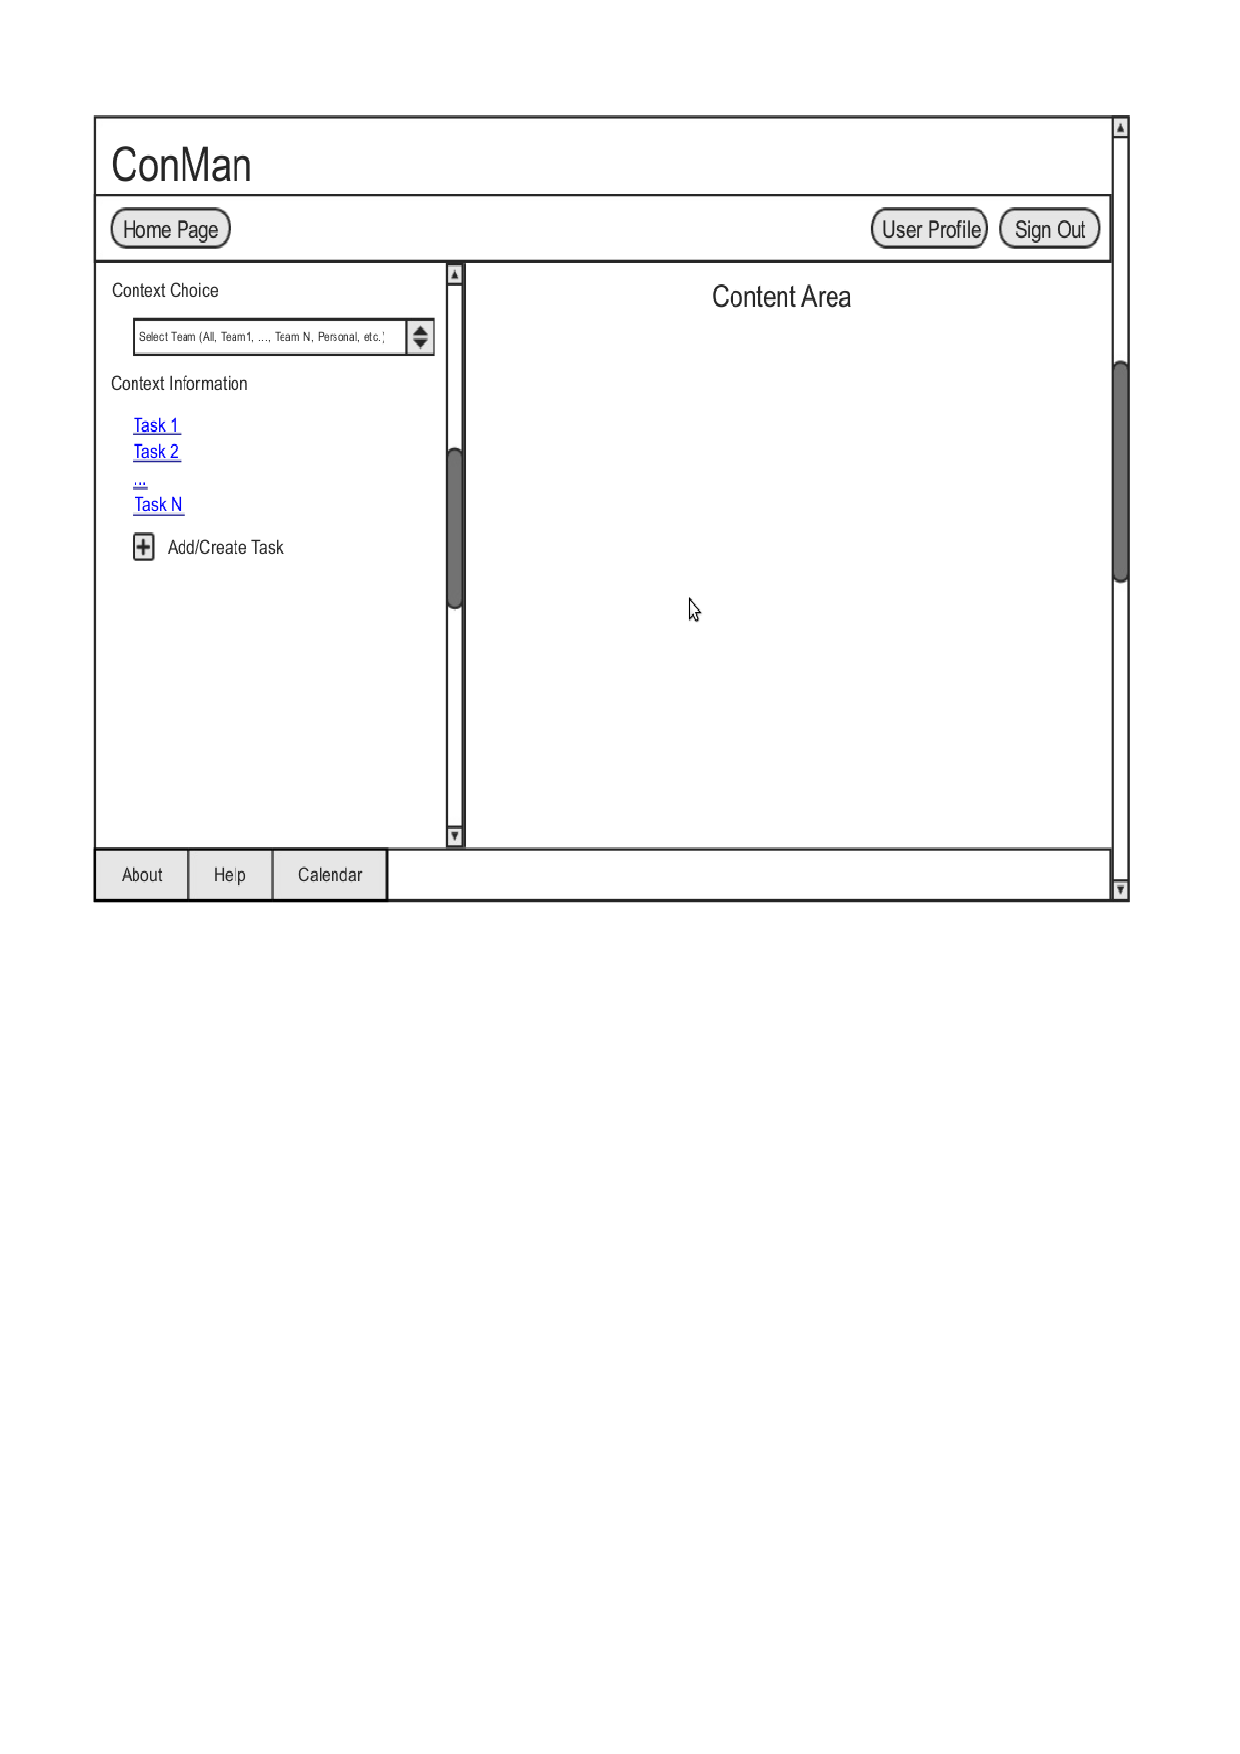
\includegraphics[trim = 0cm 14cm 0cm 0cm, clip=true, scale=0.7]{images/mainscreen}
\end{center}
As can be seen here, the top and bottom bars are populated with navigational tools.
The left pane allows the user to select which context they would like to operate in (personal or team context) and displays options relating to the selected context.
The content area then has three primary views
\subsection{Content Area}
\subsubsection{Calendar View}
\begin{center}
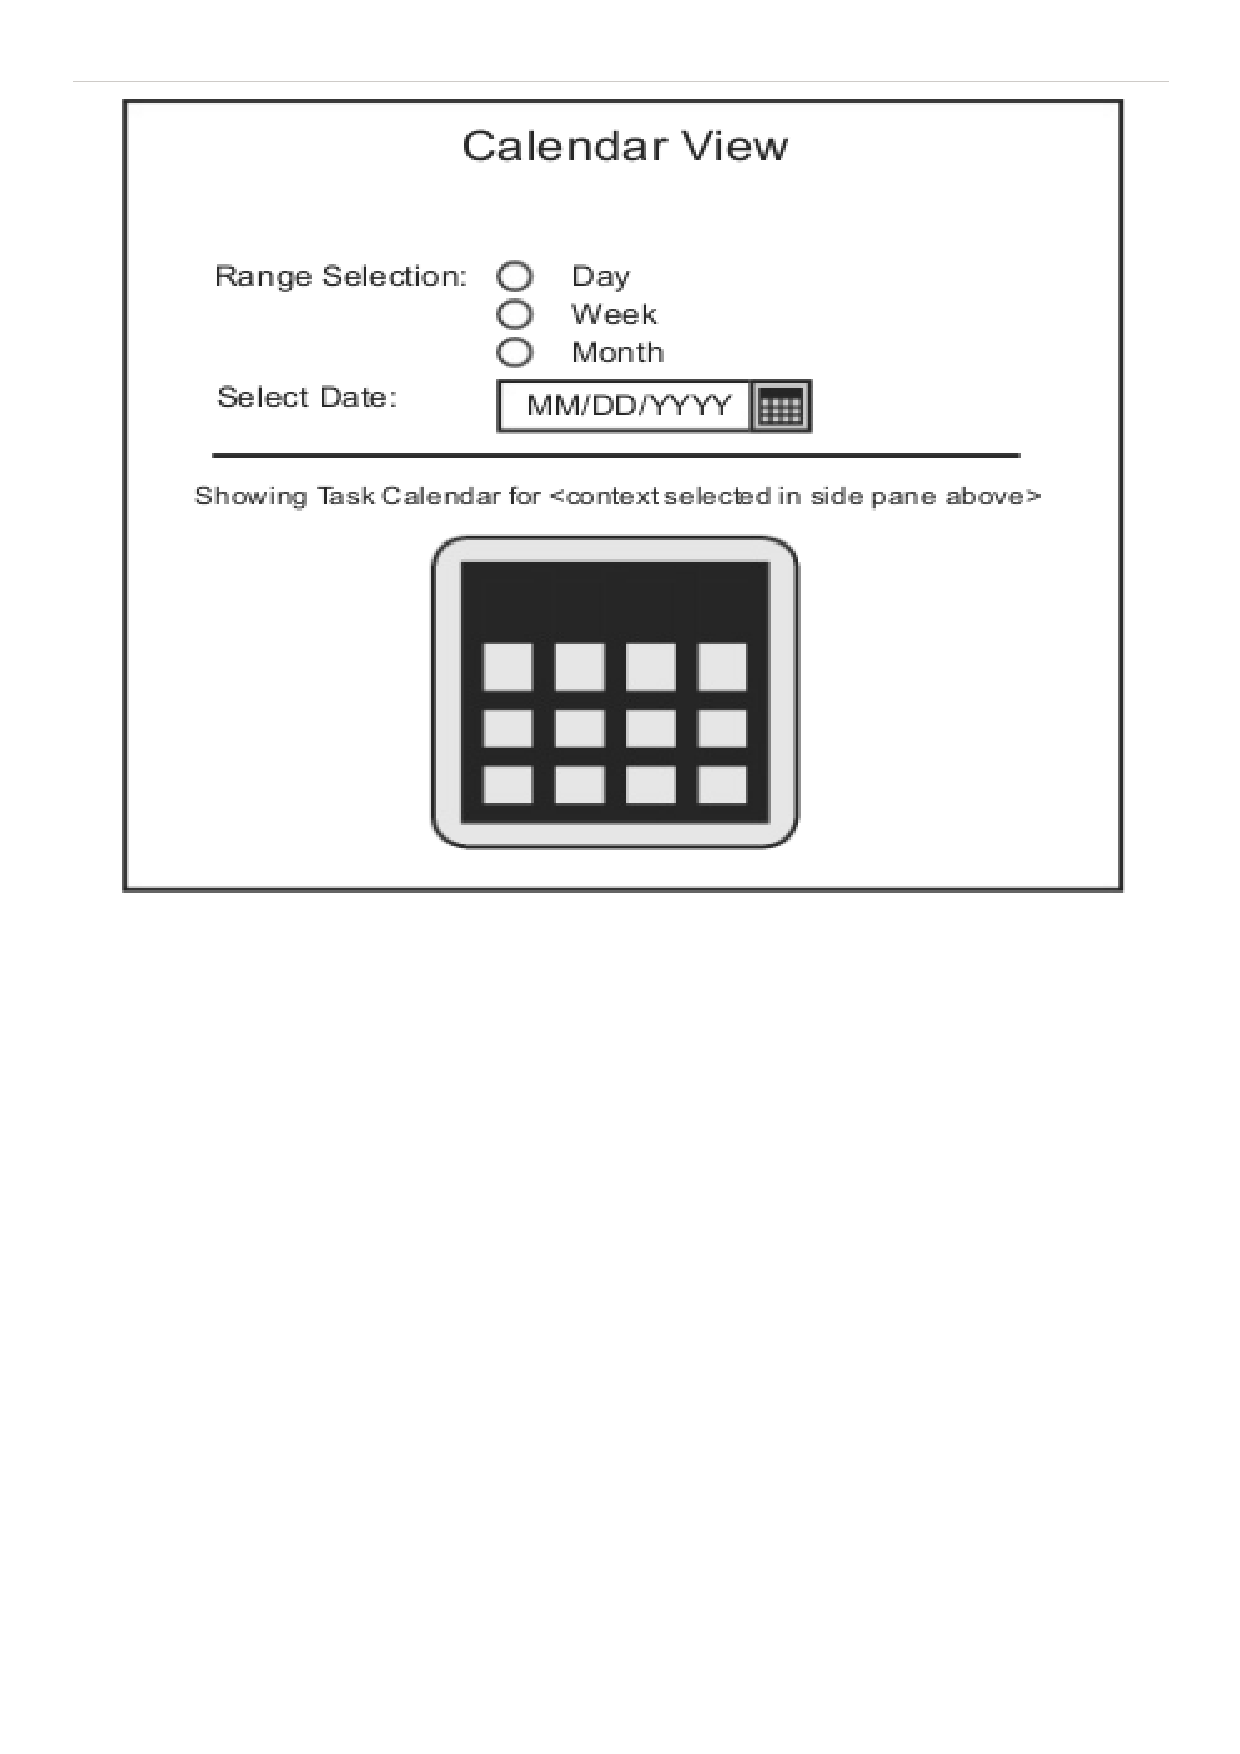
\includegraphics[trim = 0cm 14cm 0cm 0cm, clip=true, scale=0.7]{images/calendarview}
\end{center}
The calendar view gives the user an opportunity to see when the tasks and checklists are due.
If the user has selected the personal context in the left pane, then only the personal context tasks will be displayed.
The tasks and checklists appearing in the calendar will be hyper-links that navigate the content area to the task or checklist view respectively.
\subsubsection{Task View}
\begin{center}
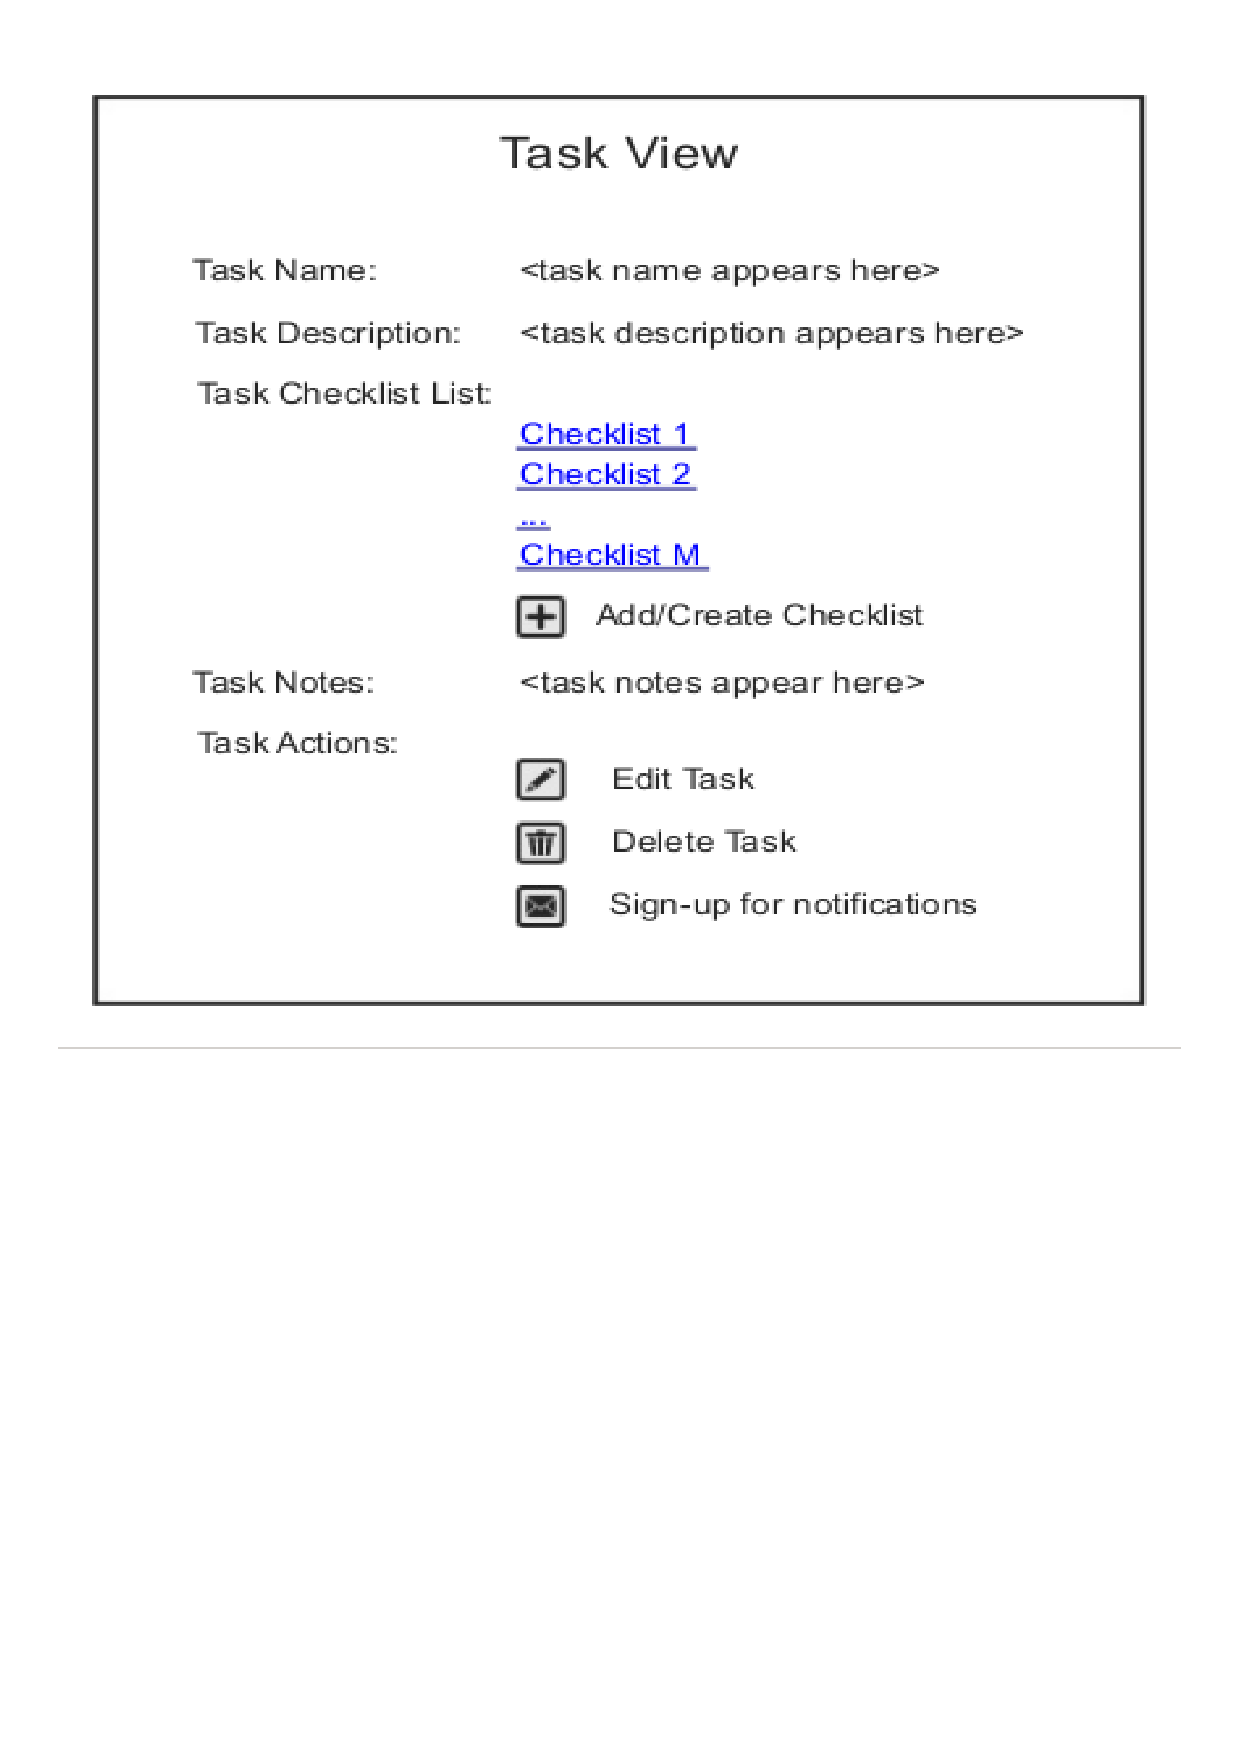
\includegraphics[trim = 0cm 12cm 0cm 0cm, clip=true, scale=0.7]{images/taskview}
\end{center}
The task view will show the task name, description, checklists, notes, and available actions for the selected task.
For tasks which are assigned to teams, non-administrative users will not be able to delete a task.
Non-administrative users will still be able to see the administrative actions, but the action link will be obscured (i.e., grayed out).
\subsubsection{Checklist View}
\begin{center}
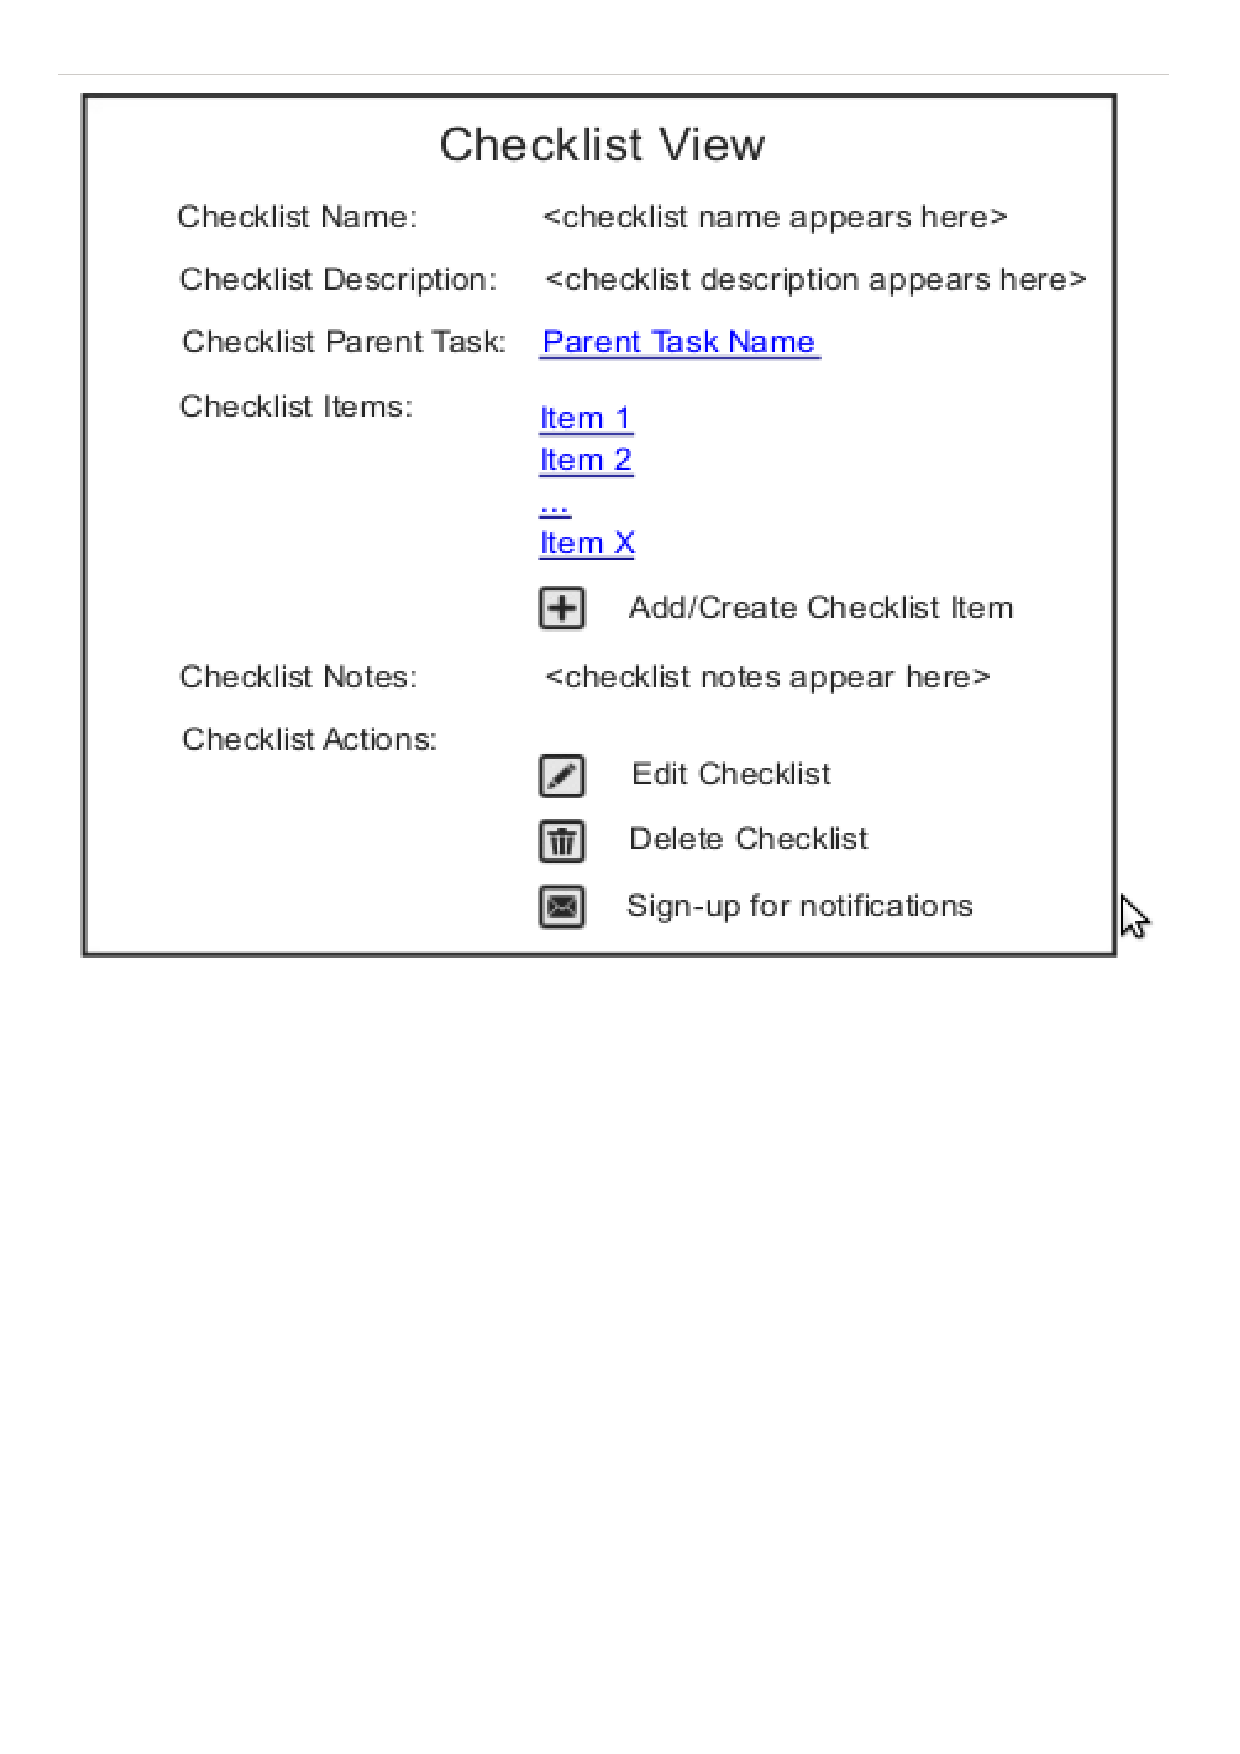
\includegraphics[trim = 0cm 12cm 0cm 0cm, clip=true, scale=0.7]{images/checklistview}
\end{center}
A checklist is conceptually very similar to a task and displays similar items.
Again, not every action will be available to non-administrative users.
\subsection{Registration Screen}
\begin{center}
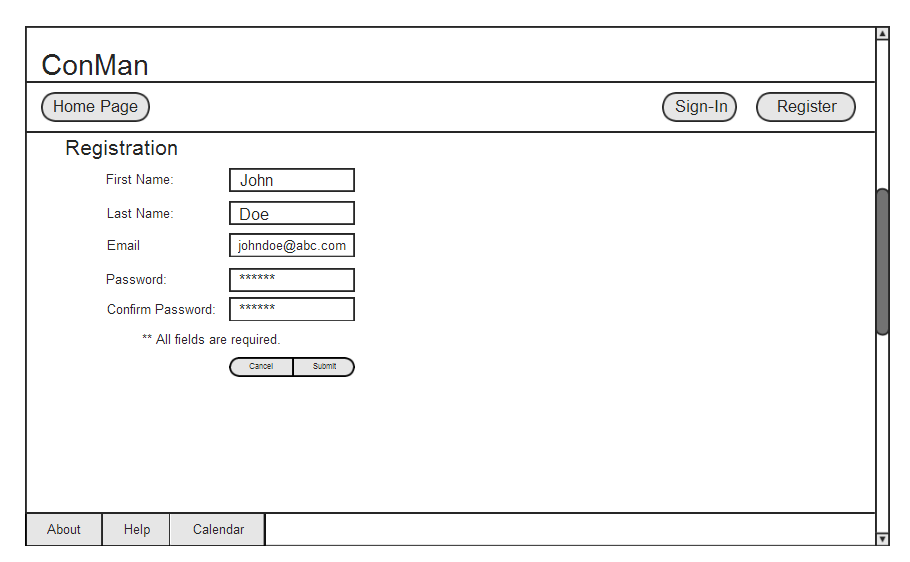
\includegraphics[trim = 0cm 0cm 0cm 0cm, clip=true, scale=0.7]{images/Registration}
\end{center}
Users must create an account for \texttt{ConMan} in order to perform a variety of function with \texttt{ConMan} 
such as registering for email notifications. Users must supply their first and last names, email, and password in 
order to register.
\subsection{Sign-In Screen}
\begin{center}
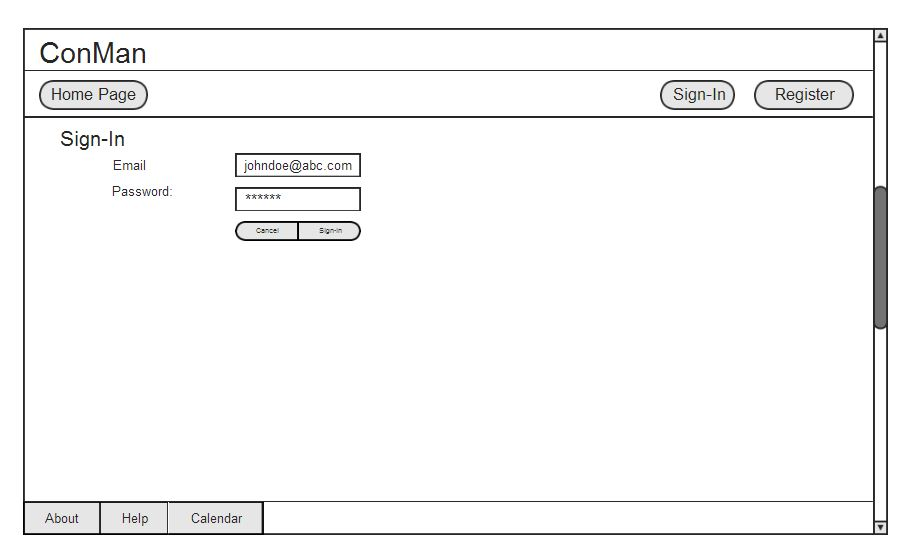
\includegraphics[trim = 0cm 0cm 0cm 0cm, clip=true, scale=0.7]{images/SignIn}
\end{center}
If an user has an account in \texttt{ConMan}, the user can sign-in using the email and 
password provided during the creation of their account.


\newpage
\section{Restrictions, Limitations, and Constraints}
As detailed in the SRS, the user interface will only be supported for the Chrome and Firefox desktop web-browsers.
Support for different browsers and devices will be added in future versions of \texttt{ConMan}.

An internet connection is also required to use \texttt{ConMan}, and there are no plans to implement off-line support.
Because \texttt{ConMan} is intended to assist coordination between teams (particularly software development teams), a network connection is essential.
\newpage
\section{Testing Guidelines}
Testing will be integrated throughout the development of \texttt{ConMan}.  Components will be tested individually before being integrated into the system for system testing.
A database of test cases, test results, and action required will be maintained by the developers to ensure \texttt{ConMan} satisfies all of its major requirements.

\subsection{Testing Cases and Expected Results}
A comprehensive test plan will ensure \texttt{ConMan} is delivered as a stable product. 
The \texttt{ConMan} tests will include tests for:
\begin{itemize}
\item account creation.  When a user creates an account the user e-mail must not already be associated with a \texttt{ConMan} account and all required fields completed.
\item account login.  When returning to \texttt{ConMan}, the user must correctly fill all required fields on the login screen.
\item team creation.  All fields associated with team creation must be completed when creating a new \texttt{ConMan} team.  E-mail fields must be properly formatted.
\item adding tasks and checklists.  When creating tasks and checklists, the user must complete all required fields.  If a due-date is required, the user must pick a date in the future.  When adding tasks to a team account, all team members must be able to view the new task.
\end{itemize}
The test-plan document will describe these and other tests in more detail.  

\newpage
\section{Appendices}
\subsection{Definitions}
\begin{itemize}
\item Client-Server: A system architecture where a central server provides data to one or many networked computers (these are the clients).
\item MVC: A design pattern commonly used for building interactive applications. The Model, View, and Controller components form the structure of the MVC pattern. The Model is a representation of  the underlying application data, the  View is a collection of objects representing the user interface elements (buttons, list, etc.), and the Controller is a connection between the Model and the View.
\item HTTP: Hypertext Transfer Protocol (HTTP) is a standard for communication between servers and web browsers.
\item URL: Uniform Resource Locator (URL) is a string of characters denoting the location of an entity (e.g., a website or an image) within the Internet.
\item JSON: JavaScript Object Notation (JSON) is a text-based standard for data interchange in a human-readable format.
\end{itemize}
\end{document}
